% Created 2020-09-22 ter 14:39
% Intended LaTeX compiler: pdflatex
\documentclass[11pt]{article}
\usepackage[utf8]{inputenc}
\usepackage[T1]{fontenc}
\usepackage{graphicx}
\usepackage{grffile}
\usepackage{longtable}
\usepackage{wrapfig}
\usepackage{rotating}
\usepackage[normalem]{ulem}
\usepackage{amsmath}
\usepackage{textcomp}
\usepackage{amssymb}
\usepackage{capt-of}
\usepackage{hyperref}
\usepackage{minted}
\usepackage[hyperref, x11names]{xcolor}
\hypersetup{colorlinks = true, urlcolor = SteelBlue4, linkcolor = black}
\usepackage[brazilian]{babel}
\usepackage{geometry}
\geometry{verbose,a4paper,left=2cm,top=2cm,right=3cm,bottom=3cm}
\author{Lourenço Bogo - 11208005}
\date{\today}
\title{Arquitetura de Computadores Lista 1}
\hypersetup{
 pdfauthor={Lourenço Bogo - 11208005},
 pdftitle={Arquitetura de Computadores Lista 1},
 pdfkeywords={},
 pdfsubject={},
 pdfcreator={Emacs 27.1 (Org mode 9.3.7)}, 
 pdflang={Brazilian}}
\begin{document}

\maketitle
\begin{enumerate}
\item Aqui estão os computadores instalados no Brasil e as informações pedidas:

\begin{center}
\begin{tabular}{rllrrr}
Posição & Nome & Instituição & \emph{Cores} & Linpack & Pico\\
56 & Atlas & Petrobrás & 91936 & 4376 & 8848.49\\
82 & Fênix & Petrobrás & 60480 & 3161 & 5371.78\\
240 & SDumont & LCNN & 33856 & 1849 & 2727.03\\
395 & Ogbon & Senai Cimatec & 27768 & 1605 & 2323.28\\
\end{tabular}
\end{center}

\textbf{OBS}: Velocidades estão e TFlop/s.

\item Com o gráfico abaixo podemos perceber que
os processadores avançam mais rápido que a memória.

\begin{center}
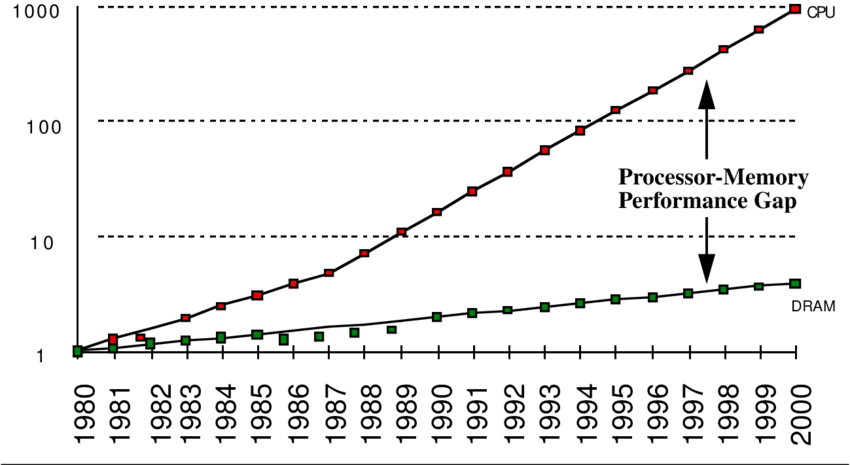
\includegraphics[width=.9\linewidth]{Processor-Memory-Performance-GapHen96.png}
\end{center}
\end{enumerate}
\end{document}